% !TEX root =  ../syst_master.tex 

\subsection{Polarization modulation efficiency}\label{subsec:modeff}

\paragraph{Description:}
The polarization modulation efficiency quantifies how much of the incident polarization signal $P_\mathrm{p,in}$ is transmitted by the HWP as $P_\mathrm{p,out}$:
\begin{equation}
\epsilon \equiv \frac{P_\mathrm{out}}{P_\mathrm{in}}
\end{equation}
in the absence of systematic effects that induce a 2f component.

With the definition above, the total intensity $I_\mathrm{out}$ at the detector can be expressed as~\cite{Matsumura:2008zx}:
\begin{equation}
I_\mathrm{out}=\frac{1}{2}\left[I_\mathrm{in}+\epsilon\sqrt{Q^2+U^2} \cos(4\chi-4\phi)\right]
\end{equation}
where $I_\mathrm{in}$ is the total incoming signal, $\chi$ is the rotation angle of the HWP, and $\phi$ is the frequency-dependent phase offset which is not relevant in the case of a monochromatic HWP.

The modulation efficiency depends on the incident frequency $\nu$, the detector bandwidth $\Delta \nu$, the incoming polarized signal $I_\mathrm{p,in}$, the incidence angle of the incoming radiation $\theta_\mathrm{i}$ and the physical properties of the HWP. In particular, the design of the HWP can be chosen in order to optimize the modulation efficiency over a broad range of frequencies. 

\paragraph{Plan to model and/or measure:}
To model the modulation efficiency, we can compute the analytic expression in the two simple cases of a monochromatic HWP (1 layer) and an achromatic HWP (AHWP, multi-layers) at normal incidence. We make use of the Mueller calculus and represent the HWP stack (arbitrary number of layers, with and without anti-reflection coating) and the detector as Mueller matrices. The Mueller matrix for the single-layer HWP takes the generic form 

\begin{equation}\label{eq:Mueller_Matrix}
M=\begin{bmatrix}
   T  &\rho  &0  &0\\
   \rho  &T  &0  &0\\
   0  &0  &c  &-s\\
   0  &0  &s  &c
\end{bmatrix}
\end{equation}

which allows for leakage off-diagonal terms. In the case of the AHWP, Eq.~\ref{eq:Mueller_matrix} takes a different form, accounting for the fact that the AHWP is a stack of several layers rotated by a certain angle with respect to the first layer. Each layer is represented by a Mueller matrix as Eq.~\ref{eq:Mueller_matrix}, and the rotation with respect to the first layer is modelled with the usual rotation matrices $R(\theta)$:
\begin{equation}
R{(2\phi)}\cdot M \cdot R(-2\phi).
\end{equation} 

The elements of the HWP (either monochromatic or achromatic) Mueller matrix are computed following the generalised transfer matrix approach~\cite{Essinger-Hileman_TM}. 

We finally model the global rotation of the HWP stack with the usual rotation matrices:
\begin{equation}
R{(2\chi)}\cdot M_\mathrm{stack} \cdot R(-2\chi).
\end{equation}

The output signal can be then analytically expressed as a series of cosine terms. The modulation efficiency is then computed as~\cite{Hanany:2005vx,Matsumura:2008zx}:
\begin{equation}\label{eq:eff}
\epsilon=\frac{A_4}{A_0}
\end{equation}
where $A_x$ is the coefficient of the n-th harmonic.

In more generic cases, including more complicated configurations, such as multi-layer stacks, slant incidence, and broad-band incident radiation, we compute the output signal at the detector following the Mueller calculus as in the analytic approach, and fit the output signal to an harmonic series of cosine terms:
\begin{equation}
I_\mathrm{out}=\Sigma_{i=0,n} A_i \cos(i\chi-i\phi).
\end{equation}

The modulation efficiency is then computed as in Eq.~\ref{eq:eff}. %\textbf{Missing an equation label somewhere}

Fig.~\ref{fig:eff} shows the polarization modulation efficiency as a function of frequency computed with the fitting procedure in two cases: a single layer HWP (curves peaking at $120\,\mathrm{GHz}$); and a 3-layer AHWP optimized to cover the two bands centered at $90\,\mathrm{GHz}$ and $150\,\mathrm{GHz}$, depicted as the gray vertical bands. It is clear that the multi-layer design is able to provide a nearly maximal polarization modulation efficiency over a broad range of frequencies. 
The different colors correspond to different incidence angles, as detailed in the legend. The modulation efficiency does not change dramatically with the incidence angle.

\begin{figure}
\begin{center}
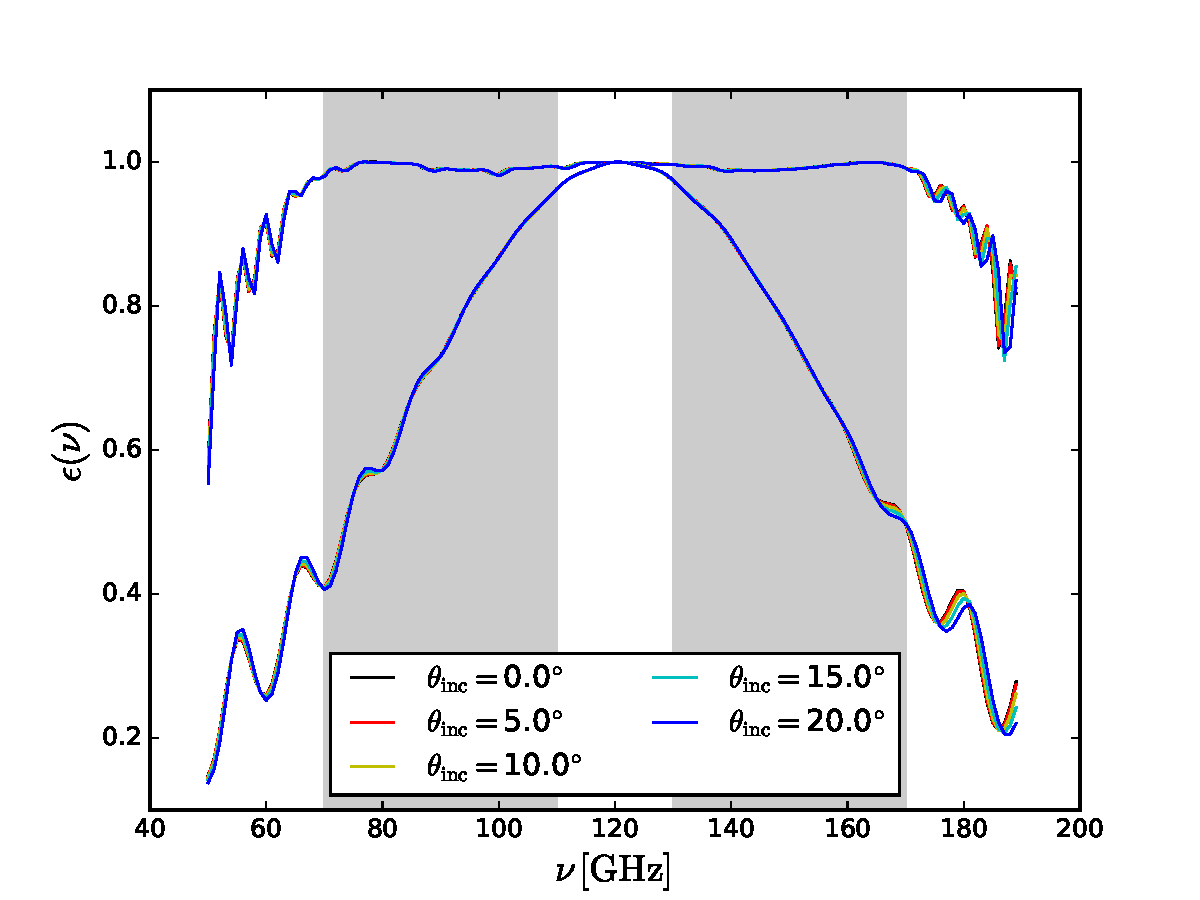
\includegraphics{figures/Eps_vs_nu_3l_PB2.pdf}
\end{center}
\caption{Polarization modulation efficiency as a function of frequency for two HWP designs: a single-layer (monochromatic) HWP centered at $120\,\mathrm{GHZ}$; and a 3-layer AHWP optimized for the two bands at $90\,\mathrm{GHz}$ and $150\,\mathrm{GHz}$. The vertical gray bands identify the two frequency bands. The different colors correspond to different incidence angles of the incoming radiation. There is not a strong dependency on the incidence angle. The assumed thickness and indexes of the sapphire are the same as in Tab.2 of~\cite{PB2a_WHWP}.}\label{fig:eff}
\end{figure}


\paragraph{Uncertainty/Range:}
The systematic effect related to the modulation efficiency is known and can be kept under control, but because it needs to be modeled, its SRF is 3.

The main systematic effect is a suppression of power in polarisation. A low modulation efficiency means that a low fraction of the polarised signal is transmitted through the HWP to the detector. In addition, what we really care about is the behaviour of the modulation efficiency over the frequency band.

For a single-layer HWP, the modulation efficiency is nearly maximal at the central frequency, and decreases rapidly otherwise. The band-averaged modulation efficiency can be therefore quite low, depending on the choice of the bandwidth.

The stacking of multiple layers of birefringent crystals allows to obtain a nearly maximal modulation efficiency over a broader range of frequencies. As an example, Fig.~\ref{fig:eff} shows the difference between a single layer HWP optimized for $120\,\mathrm{GHz}$ and a 3-layer AHWP which is optimized for the two bands at $90\,\mathrm{GHz}$ and $150\,\mathrm{GHz}$. For comparison, the band-averaged modulation efficiency for the single-layer HWP is 72\% over a 30\% frequency band centered at $90\,\mathrm{GHz}$ and 75\% for a 30\% frequency band centered at $150\,\mathrm{GHz}$. The use of a 3-layer AHWP allows to improve those figures up to a 99\% modulation efficiency over both frequency bands.

The final design of the AHWP, and in particular the choice of the number of layers which in turn sets the overall thickness of the stack, has to come as a balance between the increased modulation efficiency and the increased absorption and emission from the thicker stack of multiple layers.
%\textbf{How does this propagate into systematics? At what level does it become significant?}

\paragraph{Parameterization:}
This effect is parameterized as the modulation efficiency as a function of frequency, $\epsilon (\nu)$. The modulation efficiency can be predicted for a given design of the HWP. This prediction gives an estimate of the fraction of polarized signal that is transmitted from the HWP to the detector, or the next element in the optical chain.


%\textbf{Cite these in the text and put the references in the bibliography file}
%
%\paragraph{References:}
%The description of this systematic entry is based on the following references:
%\begin{itemize}
%\item T. Hessinger-Hileman, ``Transfer matrix for treating stratified media including birefringent crystals'', arXiv:1301.6160v3 [physics.optics], for the modelling of the HWP
%\item T. Matsumura \textit{et al}, ``Analysis of performance of three- and five-stack achromatic half-wave plates at millimeter wavelengths'', arXiv:0806.1518v1 [physics.optics], for the definition and calculation methods of $\epsilon$.
%\item S. Hanany \textit{et al}, ``A Millimeter-Wave Achromatic Half Wave Plate'', arXiv:physics/0503122 [physics.optics], for the definition and calculation of $\epsilon$ according to the fitting procedure.
%\end{itemize}
